\documentclass[10pt,twocolumn]{article}
\usepackage[letterpaper,margin=0.70in,columnsep=0.25in]{geometry}
\usepackage[T1]{fontenc}
\usepackage{lmodern,microtype,amsmath,amssymb,booktabs,graphicx,enumitem}
\usepackage[numbers,sort&compress]{natbib}
\usepackage[colorlinks=true,allcolors=blue]{hyperref}
\usepackage{url}
\setlist{nosep,leftmargin=*}
\newcommand{\LiquidSpeed}{1.75}
\newcommand{\ClefSpeed}{1.62}
\newcommand{\DeciderSpeed}{2.79}

\setlength{\parskip}{0.25em}
\title{DFIP: A Systems Study of Fidelity-Aware\protect\\Inference for Open Decision Models}
\author{Ismail Pelaseyed \qquad Alan Zabihi\\Superagent Technologies Inc.}
\date{October 12, 2026\\\small Review draft; not submitted to arXiv}
\begin{document}
\maketitle
\begin{abstract}
Open decision models return a categorical distribution, a Boolean confidence, or an ordinal score rather than a long generated response. Their inference paths nevertheless include substantial host dispatch, model-specific scheduling, and sometimes a full-vocabulary output projection. We study a decision-focused inference path (DFIP) that preserves released prompt and readout semantics while applying selective CUDA graph replay and, where applicable, candidate-token projection. We evaluate pinned checkpoints from Liquid AI, Cloudflare, Perplexity, Superagent, and Supersonic Labs on Modal GPUs. Randomized paired runs, component ablations, new diagnostic workloads derived from BANKING77, and changing-shape traces expose both useful acceleration and important limits. Retained short Boolean runs show \LiquidSpeed{}$\times$ for d1-3B, \ClefSpeed{}$\times$ for Clef, and \DeciderSpeed{}$\times$ for PPLX-Decider; the first two condition on three of five planned rounds. Graph replay is the principal source of improvement; candidate projection alone does not establish a general speedup. In each completed fidelity evaluation of 3,024 decisions, the tested policies preserve the winning answer but do not uniformly preserve probabilities. A candidate-head experiment on Security-One illustrates why probability drift must be checked independently of decision agreement. GPU errors also prevent a complete repeated-run result for Julia-1 and cause attrition for two checkpoints. We release raw timing samples, failure traces, pinned model and dataset revisions, and analysis code. This draft presents a bounded systems characterization, not a new general graph algorithm or a production serving benchmark.
\end{abstract}

\section{Introduction}
Routing, policy classification, and structured scoring often require a small answer set. In these applications, inference returns a decision distribution rather than an open-ended continuation. A deployment can therefore spend much of its request time on tokenization, Python dispatch, GPU launch overhead, and output computation whose results are discarded. Reducing this work is attractive for both latency and compute cost, but the relevant contract includes calibrated probabilities and ordinal scores as well as the winning label.

Existing serving systems already support structured programs and constrained selection. SGLang, for example, includes a selection primitive and exploits execution structure in its runtime~\citep{sglang}. CUDA graphs and compiler transformations likewise provide established tools for reducing launch overhead~\citep{pygraph,cudagraphs}. DFIP does not introduce these ideas. Our question is how far a small, model-aware implementation can apply them to recently released open decision checkpoints without silently changing their interfaces or numerical behavior.

We ask three research questions. \textbf{RQ1:} Which released inference paths benefit from selective replay under short, long, batched, and multi-question workloads? \textbf{RQ2:} How much improvement comes from graph replay versus candidate projection? \textbf{RQ3:} Which optimizations preserve decision and probability behavior, and where do they fail? Our contribution is a reproducible implementation and empirical characterization with negative results, rather than a universal acceleration claim.

The artifact is available for author review at \url{https://github.com/superagent-ai/dfip}. At this draft stage the repository is private; public artifact access and a frozen release must be resolved before submission. The implementation uses Python for adapters, validation, and orchestration, and Triton~\citep{triton} for experimental GPU kernels. All checkpoints and benchmark datasets remain on Modal; a lightweight local client sends structured requests.

\section{Decision Contracts and Scope}
An input contains a state $s$ and a set of typed questions $Q$. A choice question returns probabilities over a finite set of criteria; a Boolean question returns a confidence in the affirmative answer; an ordinal question returns a distribution over ordered levels and may expose its expected score. The checkpoints implement these contracts using different prompt encodings and different heads. A common client interface does not imply interchangeable internal computation.

Julia-1 uses a ModernBERT-based encoder and marker-oriented decision readout. Liquid's d1-3B uses its released LFM-based engine, including a packed trunk/branch path for multiple questions. Clef-Flash uses a Qwen backbone and a joint schema head. PPLX-Decider uses its released Qwen-based decision model. Security-One is evaluated through its SGLang path~\citep{julia,liquid,clef,decider,security}. We retain each released prompt construction, candidate ordering, alias handling, temperature, and answer conversion. We do not train, quantize, or distill the checkpoints.

These are five selected checkpoints, not an exhaustive sample of the Hugging Face decision-model tag. Text-only workloads are tested even when a checkpoint supports images. Tests do not establish safety, deployment suitability, or superior task quality. We also do not compare with generic one-token generation as though it were a semantically identical baseline.

\subsection{When candidate projection is valid}
Let $h\in\mathbb{R}^{d}$ be the hidden vector at a released answer position and $z=Wh$ the vocabulary logits. For a native readout that groups answer-token aliases $A_c$, a representative contract is
\begin{equation}
 r_c=\max_{t\in A_c}z_t,\qquad
 p_c=\frac{\exp(r_c/\tau)}{\sum_j\exp(r_j/\tau)}.
\end{equation}
If $U=\bigcup_c A_c$, computing $W_Uh$ preserves these readout logits in real arithmetic. A common log-normalization constant cancels when the selected scores are subsequently normalized over candidates. The condition is that the released readout consumes only the covered token groups: arbitrary generation, a full-vocabulary confidence, top-$k$ operations over the entire vocabulary, or an incomplete alias union do not satisfy it. Other decision heads need their own contract analysis.

This identity is not a finite-precision equivalence theorem. A smaller matrix multiply can choose a different reduction order or precision path. If $\|p-\hat p\|_\infty\leq\epsilon$, an argmax with a margin greater than $2\epsilon$ is preserved, while a threshold comparison at $a$ is preserved only when $|p_c-a|>\epsilon$. For ordinal levels $v_c$, expected-score drift is bounded by $\sum_c |v_c|\,|p_c-\hat p_c|$. Agreement of the winning label alone is thus insufficient for probability-sensitive applications.

\section{Implementation}
\subsection{Adapters and selective graph replay}
The runtime loads an immutable checkpoint revision and uses an adapter to invoke the released inference engine. DFIP wraps a compatible forward boundary with static input buffers and a shape cache. A key records tensor dimensions, strides, dtype, device, and supported scalar metadata. Replays copy current inputs into the captured buffers; the cache stores computation, never a previous prediction. Calls sharing mutable buffers are serialized in the serving engine.

The v1 tested policy admits a shape after three encounters and bounds the graph cache to four entries. Liquid, Clef, and PPLX-Decider use a 512-token capture limit. Clef and PPLX-Decider limit capture to a single forward row. Unsupported paths use the released native implementation. A hybrid recurrence path additionally keys valid lengths, since shape equality alone cannot prove control-flow equivalence. For Julia, an equivalent local attention mask is constructed on the GPU to make capture possible. These adaptations are implementation choices rather than claims of novel graph scheduling.

Captured allocation lifetime is another constraint. The first expanded protocol encountered illegal GPU memory access in three checkpoint applications. The error was observed during benchmark execution, sometimes after a mode transition; asynchronous reporting does not identify the responsible kernel. Failure excerpts are retained. A follow-up implementation synchronizes before clearing or evicting a graph. A 60-call synthetic-kernel test covering shape eviction and cache clearing passes, but Julia still fails during the new-workload fidelity run after this change. This does not resolve the model-level failure, and we do not pool the follow-up with the original protocol. The review branch therefore defaults Julia, Liquid, and Clef to released native inference pending broader validation; PPLX-Decider retains its bounded graph policy and Security-One retains native SGLang. Existing deployed applications were not changed.

\subsection{Candidate heads and rejected kernels}
For d1-3B, the adapter derives answer-token groups using the released tokenizer and readout code. A head projects the verified union with either a Triton reduction kernel or PyTorch's linear operation. New groups extend that union and invalidate existing captures. To preserve the released engine's tensor interface, the current prototype reconstructs a vocabulary-shaped tensor with uncomputed positions set to negative infinity. It therefore removes much projection arithmetic but retains output allocation, scatter, and readout overhead. This is an explicit limitation rather than a minimal-width output implementation.

Security-One's experimental SGLang patch projects its verified answer-code rows at the native output boundary. It is isolated from the selected deployment policy, which remains native SGLang. The comparison uses both Triton and cuBLAS-backed projection. Experimental RMSNorm replacements and released compiler options from the earlier development study are retained as supplementary evidence. They are not enabled merely because a local kernel test passes: full-model probability and decision checks determine whether a path is admissible.

\subsection{Modal execution and packaging}
GPU workers use pinned model revisions and persistent remote volumes. The local package depends on the Modal client, not PyTorch or checkpoint weights. It exposes preparation, deployment, inference, and validation commands, while accelerator dependencies live in remote images. Deployment can scale to zero. The study initially ran model applications concurrently and reached the workspace's GPU concurrency limit; subsequent workers are capped at one container, and follow-up experiments are serialized. Concurrency changes how quickly experiments finish and is not a source of model acceleration.

\section{Experimental Method}
\subsection{Hardware, software, and baselines}
Julia, d1-3B, and Clef run on one NVIDIA L40S each; PPLX-Decider and Security-One run on one NVIDIA B200 each. Worker requests use four CPU cores and 32~GiB of host memory for the smaller models, and eight cores and 96~GiB for the larger models. Per-round GPU identity, driver, CUDA version, package versions, and container identity accompany the raw samples. The Transformers reference images use PyTorch 2.14.0, CUDA 13.0, Triton 3.8.0, and Transformers 5.17.0; Julia uses Transformers 5.0.0. Security-One uses the SGLang 0.5.19 CUDA 13 image.

The primary baseline is the released eager/native adapter in the same environment. This is not a comparison against every optimized serving engine. In particular, the initial Qwen reference environment lacks the optional \texttt{causal-conv1d} extension and uses a PyTorch fallback. An optional extension build is recorded separately; results from such a build must not be mixed with the fallback baseline. Consequently, gains for Clef and PPLX-Decider cannot be interpreted as improvements over an optimized-kernel ceiling. SGLang already supplies an optimized serving substrate for Security-One.

\subsection{Workloads and fidelity sets}
Nine timing workloads cover a short Boolean decision, a short categorical decision, three questions on one state, medium and long repeated-log contexts, candidate widths 2, 8, and 16, and eight requests in one batch. The exact states and schemas are defined in the artifact. Contexts are synthetic; token counts differ across released prompt encodings. A 120-call trace changes state content and lengths across 40 context sizes to test admission and replay without prediction caching.

The first fidelity set contains 400 typed-decision cases with 2,000 questions from the pinned \texttt{LocalLLaMA/typed-decisions} test split. This set was used during earlier DFIP development and is not a pristine holdout. A second workload samples 256 test utterances from BANKING77~\citep{banking}. For each utterance, we construct one single-choice record and one record containing choice, Boolean, and ordinal questions: 512 records and 1,024 decisions in total. Choice candidate widths cycle through 2, 4, 8, and 16 and include the gold intent. Boolean targets alternate between matching and nonmatching intents. Derived ordinal questions are diagnostic and have no validated annotation. Dataset revision hashes, content checksums, seeds, and generated-record hashes are included. Checkpoint training overlap with either corpus is unknown.

We compare complete returned probability distributions, winning labels, expected ordinal scores, and probability-slot threshold crossings at 0.1, 0.25, 0.5, 0.75, and 0.9. Clef rounds probabilities in its released API, so measured drift is at that interface rather than an unrounded internal-logit claim. Diagnostic accuracy, Brier score, and equal-width expected calibration error are available for the derived choice/Boolean labels, but repeated single-choice and multi-question views of one utterance are correlated. They are not independent quality examples.

\subsection{Timing and statistical unit}
The protocol plans five independent single-use container rounds per checkpoint, with 50 timed calls per workload and mode after four admission/warmup calls. Mode and workload orders are randomized by round. GPU synchronization brackets the resident Transformers API timing, which includes encoding, forward computation, and native readout. Security-One timing includes the in-container HTTP client and SGLang scheduler. It excludes external client networking and server startup. Its native runs bracket the randomized head experiments to expose drift across server restarts.

The statistical unit is a container round. We compute each workload's median within each round, pair native and tested-policy medians, and report their geometric-mean ratio. Intervals are 95\% percentile bootstrap intervals over paired log ratios with 10,000 resamples; the 50 calls are not treated as 50 independent deployment replications. Small samples and cloud variability remain limitations. For Security-One, the within-round reference is the geometric mean of the two native medians.

Julia's initial application returned no complete expanded-protocol round. Liquid and Clef each returned three rounds before an application-level GPU error aborted the remaining work. PPLX-Decider and Security-One completed five rounds each. Security-One's last container also emitted driver graphics-exception warnings before the first measured mode; the function continued and returned a complete round. We retain these warnings without assigning a kernel root cause. Tables are generated from complete retained JSON records and report actual counts. Attrition can be nonrandom, so intervals based on retained runs are conditional and may be optimistic. We do not impute failed rounds or substitute old one-container samples as independent repetitions.

\section{Results}
\subsection{RQ1: Workload-dependent acceleration}
Table~\ref{tab:latency} reports the short Boolean workload, while Figure~\ref{fig:workloads} covers all nine shapes. These are experimental v1 policies; the review branch uses native defaults for paths that failed expanded validation. The main pattern is that repeated short requests benefit more than long, batched, or multi-question paths. The tested policy deliberately falls back when capture is unsupported; different internal paths also explain why a single model-wide speedup is misleading.

\begin{table*}[t]
\centering\small
\begin{tabular}{lrrrr}
\toprule
Checkpoint & Complete rounds & Native median (ms) & Tested median (ms) & Paired speedup [95\% CI] \\
\midrule
Julia-1 & 0 & -- & -- & GPU error \\
d1-3B & 3 & 18.69 & 10.68 & 1.75 [1.26, 2.07] \\
Clef-Flash & 3 & 61.06 & 37.77 & 1.62 [1.60, 1.66] \\
PPLX-Decider & 5 & 95.55 & 34.23 & 2.79 [2.17, 3.23] \\
Security-One & 5 & 37.94 & 38.74 & 0.98 [0.90, 1.04] \\
\bottomrule
\end{tabular}

\caption{Short Boolean request. Latencies are geometric means of container-level medians. Liquid/Clef intervals condition on three of five planned rounds. Security-One tests the experimental Triton head against bracketing native SGLang; the selected deployed path remains native. Julia's initial expanded protocol failed rather than yielding a repeated-run estimate.}
\label{tab:latency}
\end{table*}

\begin{figure*}[t]
\centering
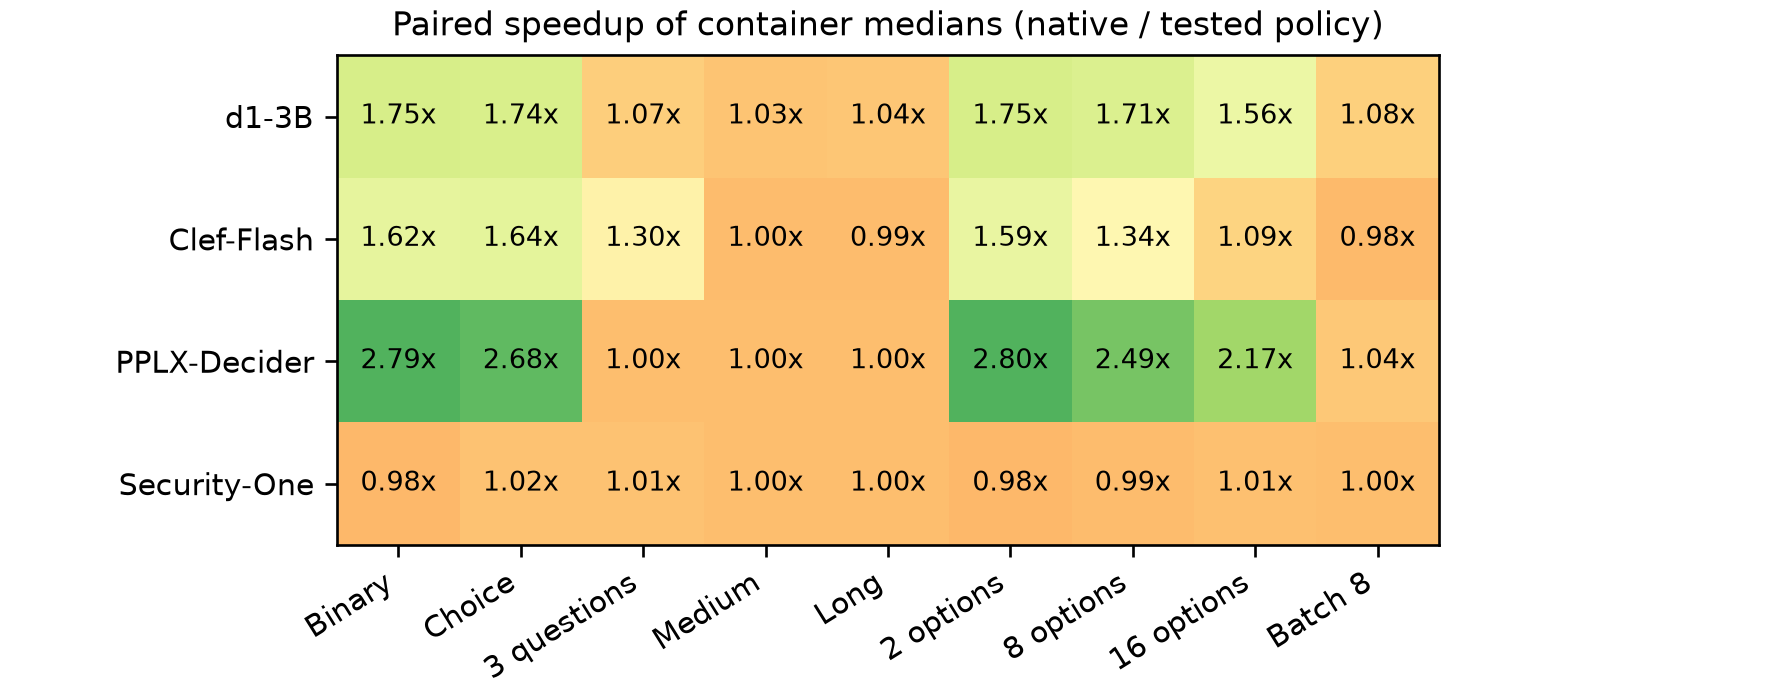
\includegraphics[width=0.98\textwidth]{generated/workloads.png}
\caption{Paired resident-API speedup across workloads. Values below 1 indicate a slowdown. Security-One is a head experiment, not the selected deployed policy. The plot excludes Julia because its initial expanded run failed. Per-round samples and conditional intervals for every cell are in the artifact.}
\label{fig:workloads}
\end{figure*}

The native baselines themselves vary across containers. Pairing measurements avoids dividing unrelated cloud runs, but it does not eliminate within-round mode-order effects, thermal or clock changes, or software allocator history. The Security-One native-before/native-after comparison is particularly useful for avoiding attribution of such variation to an output-head patch. These results describe resident serial-call latency; reciprocal latency is a serial service-rate estimate, not measured concurrent serving throughput.

\subsection{RQ2: Graph replay versus projection}
Table~\ref{tab:ablation} isolates the d1-3B components on the short Boolean workload. Graph-only replay supplies the large part of the observed reduction. Candidate projection without replay does not establish a general gain, and changing between cuBLAS and Triton within the graphed path gives a much smaller difference. This is consistent with a request whose total time also contains encoding, backbone execution, and Python readout.

\begin{table}[t]
\centering\small
\begin{tabular}{lrr}
\toprule
d1-3B mode & Median (ms) & Speedup [95\% CI] \\
\midrule
\texttt{native} & 18.69 & 1.00 [1.00, 1.00] \\
\texttt{graphs\_only} & 11.47 & 1.63 [1.18, 1.92] \\
\texttt{candidate\_cublas} & 18.40 & 1.02 [0.95, 1.07] \\
\texttt{candidate\_triton} & 18.12 & 1.03 [1.00, 1.06] \\
\texttt{production\_cublas} & 10.69 & 1.75 [1.26, 2.08] \\
\texttt{production} & 10.68 & 1.75 [1.26, 2.07] \\
\bottomrule
\end{tabular}

\caption{Short Boolean ablation, three retained paired rounds. \texttt{production} combines graph replay and the Triton candidate head. The dynamically extended union contains 40--42 tokens during these timing observations; that order-dependent detail limits a strict fixed-width kernel interpretation.}
\label{tab:ablation}
\end{table}

This ablation supports retaining a model-aware replay path but does not support marketing DFIP as a generally faster custom matrix-multiply kernel. The prototype still reconstructs a vocabulary-shaped output. A narrower readout interface and comparison with fully optimized native kernels are separate engineering and experimental questions.

\subsection{RQ3: Decision agreement is weaker than fidelity}
Table~\ref{tab:fidelity} combines the two fidelity sets for complete round-zero results. No tested policy in the table changes a winning decision or crosses the five sampled probability thresholds. Nevertheless, d1-3B and Clef exhibit measurable drift on the new workload. The absence of crossings at these five thresholds does not establish safety for arbitrary thresholds close to a model confidence, and exact real-arithmetic projection does not imply bitwise equality.

\begin{table}[t]
\centering\small\setlength{\tabcolsep}{3pt}
\begin{tabular}{lrrrr}
\toprule
Checkpoint & Decisions & Flips & Crossings & Max $|\Delta p|$ \\
\midrule
Clef-Flash & 3024 & 0 & 0 & 0.0062 \\
PPLX-Decider & 3024 & 0 & 0 & 0 \\
d1-3B & 3024 & 0 & 0 & 0.00738 \\
Security-One & 3024 & 0 & 0 & 1.82e-07 \\
\bottomrule
\end{tabular}

\caption{Released-API fidelity for retained complete round zero: 2,000 typed questions plus 1,024 derived BANKING77 decisions per checkpoint. Crossings count probability slots over all five thresholds. Security-One uses the experimental Triton head. This is empirical agreement, not an all-input guarantee.}
\label{tab:fidelity}
\end{table}

The Security-One cuBLAS-backed candidate head provides a clear counterexample to using label agreement as the only gate: it preserves all 2,000 winning labels in the typed set but reaches a maximum probability difference of approximately 0.0393. The Triton variant is much closer to the native probabilities, with a maximum difference below $2\times10^{-7}$ on that set. Neither result proves that candidate projection yields a worthwhile full-request speedup on the SGLang substrate. The selected deployment therefore retains native SGLang. A separate single-container Clef follow-up with the optional native convolution extension also preserves winning labels, but produces two sampled threshold crossings and a maximum new-workload probability difference of 0.0129 (Appendix~\ref{app:followup}). This is a concrete probability-sensitive failure even when argmax agreement is complete.

Earlier exploratory RMSNorm substitutions changed winning labels for Liquid, Clef, and PPLX-Decider, and a Julia compiler experiment changed decisions as well. Those observations motivated the full-model gates and are archived separately from the repeated-run protocol. Kernel-level closeness to a reference reduction is insufficient: changed accumulation and rounding can propagate through many layers or a calibrated readout. The original expanded run's GPU failures similarly prevent a blanket reliability claim about all replay shapes.

\section{Cost Interpretation and Deployment Limits}
At Modal's listed rates on October 12, 2026, an L40S costs \$0.000542 per GPU-second and a B200 costs \$0.001736~\citep{modalpricing}. A narrow compute estimate for $D$ decisions per call is
\begin{equation}
 C_{1000}^{\mathrm{GPU}}=1000\,r_{\mathrm{GPU}}\,T_{\mathrm{call}}/D,
\end{equation}
where $T_{\mathrm{call}}$ is in seconds. The artifact computes this quantity from the retained medians. It is not a measured invoice or a cost-per-request claim for a network service. CPU, memory, model loading, graph admission, idle container lifetime, storage, networking, and plan fees are excluded.

For $N$ calls within one billed container lifetime, a more useful approximation is
\begin{equation}
 C\approx r_{\mathrm{resources}}
 (T_{\mathrm{load}}+T_{\mathrm{admit}}+NT_{\mathrm{serve}}+T_{\mathrm{idle}}).
\end{equation}
Modal bills load and processing time and the configured idle window~\citep{modalpricing}. For sparse traffic these terms can dominate a small kernel reduction. Capping benchmark concurrency avoids a plan upgrade but does not make a fixed amount of GPU work free. A production claim would require external-network latency, arrival-process experiments, queueing and tail-latency measurements, observed resource consumption, and invoice reconciliation. None is established by the resident serial benchmark here.

\section{Related Work}
SGLang~\citep{sglang} combines structured language-model programs with a runtime that reuses execution structure. DFIP uses a narrower native decision contract and does not claim structured selection as a new primitive. PagedAttention and vLLM~\citep{vllm} address KV-cache memory management and serving throughput for generation; those mechanisms and their arrival-rate evaluation are distinct from this serial decision-path study.

PyGraph~\citep{pygraph} develops compiler support for robust CUDA graph use and evaluates component contributions across workloads. Its broader treatment makes clear that a small shape cache is not a novel graph compiler. PyTorch's CUDA graph documentation~\citep{cudagraphs} also specifies static-address and control-flow constraints. Triton~\citep{triton} provides a tiled programming model for custom GPU computation; DFIP applies it to a small candidate projection rather than proposing a new language or tensor primitive.

MLPerf Inference~\citep{mlperf} emphasizes workload scenarios, quality constraints, and latency/throughput measurement. This informs our separation of fidelity from timing, but the present study is not MLPerf-compliant and does not measure all of its serving scenarios. BANKING77~\citep{banking} supplies an independently sourced intent workload; deriving a finite candidate set from its labels is our diagnostic construction, not the original benchmark task or a new validated scoring dataset.

\section{Threats to Validity and Open Work}
\textbf{Baseline strength.} Optional native convolution kernels are absent in the initial Transformers environment. Baselines are model-release adapters, not a tuned comparison against all serving engines. \textbf{Selection and attrition.} Five checkpoints are chosen for interface diversity. Failed rounds are not missing at random, and three-round conditional intervals provide weak evidence of population stability. Julia lacks a complete initial expanded-protocol result.

\textbf{Workload validity.} Timing states are synthetic and resident calls have little arrival-process diversity. BANKING77 schemas are derived, and duplicated utterance views are correlated. The typed set was used during development, and checkpoint training overlap is unknown. Image paths, adversarial states, maximum supported contexts, multi-GPU configurations, and production concurrency are untested here.

\textbf{Numerical validity.} Returned probabilities may be rounded, calibration magnifies some logit differences, and five threshold values cannot cover all application policies. No observed label flip is a finite sample statement. Dynamic candidate coverage and graph admission interact with workload order. The initial failure's asynchronous traceback cannot establish a kernel-level root cause, and a conservative synchronization change requires independent validation.

\textbf{Reproducibility.} Model and dataset revisions and package versions are recorded, but cloud scheduling, hardware contention, driver updates, transitive dependencies, and graph-library behavior are not fully controlled. Fresh containers do not guarantee independent physical hosts. The artifact preserves source versions and failed runs. Before an arXiv submission, the authors should review the failures, complete the optimized-baseline and external serving comparisons if they wish to make stronger claims, freeze a public artifact, and check every generated table against the archived results.

\section{Conclusion}
DFIP shows how a lightweight, model-aware decision inference implementation can combine native semantics with established replay and candidate-readout techniques. The retained results favor selective graph replay for repeated short workloads and provide weaker evidence for custom output projection as a full-request optimization. Probability drift and GPU failures define meaningful boundaries of the current prototype. A useful research contribution is therefore the characterization and reproducible evidence, including rejected paths, rather than an unconditional promise of faster or exact inference across decision models.

\bibliographystyle{plainnat}
\bibliography{references}

\appendix
\section{Artifact and Reproduction}
The repository contains a pinned model registry, remote preparation code, research entry points, raw per-call timing JSON, derived-workload generation, failure excerpts, and deterministic analysis. \texttt{scripts/analyze\_paper.py} regenerates the tables and workload plot directly from complete retained records. Its checks reject inconsistent medians and malformed timing samples. A source archive preserves the first protocol's implementation separately from follow-up lifetime changes.

The local client does not download checkpoints or corpora. Reproduction requires a Modal workspace and sufficient access to the referenced model repositories. Execute one checkpoint application at a time with at most one GPU container. The default research worker cap is one. Five rounds are planned; failures should be retained as outcomes rather than excluded without explanation. Any follow-up optimized-extension baseline or synchronized replay run lives in a separate result namespace.

The LaTeX source is built with \texttt{latexmk -pdf main.tex}. A CPU-only Modal typesetting entry point is supplied when TeX is unavailable locally. The review artifact includes the source and generated figures; arXiv submission has not been performed.

\section{Checkpoint and Dataset Identity}
Full checkpoint SHA revisions are in \texttt{src/dfip/models.py}. The typed corpus revision is \texttt{c76749ec58bd8c3d2ea706b31c333a9059c38f90}; the BANKING77 revision is \texttt{8eed2b348ec07d40ffbe91dcc4718e2f0f977714}. Data checksums are verified by remote loaders, and the derived records use random seed 20261012. Per-container package manifests must be consulted rather than assuming all checkpoints share one environment.
\section{Separate Follow-up Experiments}\label{app:followup}
The synchronized-retirement follow-up uses source commit \texttt{b8f028d57a499e29736585675b13b02a034351af} and a separate result namespace. Its GPU kernel checks pass, including 60 changed-shape calls with a four-entry cache, eviction, and clearing. Julia still fails during the derived-workload run; synchronization alone does not establish model-level robustness.

An exploratory Clef container with \texttt{causal-conv1d} 1.7.0 installed completes all workloads and fidelity checks. Its short Boolean native median is 60.31\,ms and its graphed median is 37.10\,ms, a paired 1.63$\times$ ratio. This is one container, without a confidence interval, and is not pooled into Table~\ref{tab:latency}. It does not establish a causal comparison between extension installation and the earlier fallback image, since environments and containers differ.

The typed fidelity set has no label or probability changes in that follow-up. On the 1,024 derived BANKING77 decisions, the graph path has zero winning-label flips but maximum probability drift 0.0129 and maximum expected-score drift 0.0189. One probability slot crosses 0.1 and another crosses 0.25. The exact IDs and probabilities are archived alongside native and graphed predictions. The 120-call changing-shape trace preserves labels with maximum probability drift 0.0012. These findings strengthen the distinction between decision agreement and probability fidelity; they do not justify enabling the experimental path by default.
\end{document}
